\chapter{Explosive percolation}

\resp{Lorenzo Rizzi}



\section{Percolation theory and phase transitions}

Percolative processes were initially introduced on specific and regular networks (e.g. $D$-dimensional lattices) to model physical phenomena such as percolation of water in porous stones. However, nothing prevents us from applying the percolation's paradigm to arbitrary network topologies. Defining $p$ as the probability that a randomly chosen edge (or node) is removed from the network, then a classical result from percolation theory is that, for certain network topologies, a phase transition (PT) occurs as $p$ is varied. If we define $S$ as the probability that a randomly chosen node belongs to the GCC (our \textit{order parameter}), then, for $N \to \infty$ (\textit{thermodynamic limit}), we have $S = 0$ for $p < p_c$ and $S = S(p) \neq 0$ for $p > p_c$.

It is a standard result \cite{Li_2021} that classical random percolation on networks displays a \textit{continuous} phase transitions, meaning that, at criticality, $S(p_c) = 0$ and the order parameter has no discontinuous behaviour around the critical point. In addition, there are various other indicators of an incoming phase transition widely used in statistical mechanics. We'll define $n_s$ as the number of (finite) clusters of size $s$ per node and $\chi$ as the average cluster size:
\begin{equation}
	\chi = \frac{\sum_s n_s s^2}{\sum_s n_s s}
\end{equation}
In second order PT, at criticality $\chi$ is expected to diverge with a well-defined critical exponent $\chi \sim |p-p_c|^{-\nu}$ and the cluster distribution $n_s$ reduces to a power law $n_s \sim s^{-\tau}$.
 
However, in 2009, an inspiring article from Achlioptas et al. ~\cite{Achlioptas} proposed a new type of percolation process that, allegedly, leads to a discontinuous type of transition (called \textit{explosive percolation} for its abrupt nature). However, posterior papers \cite{cont} have managed to prove that explosive percolation is actually a continuous one. In the present task, we are going to explore and simulate Achlioptas process(es) on various network topologies to recreate the explosive percolation behaviour.
\label{par::intro}

\section{Achlioptas processes on random graphs}
\label{par:Achlioptas}
Classical percolation prescribes the removal (or addition) of randomly selected edges (or nodes). As mentioned in Par \ref{par::intro}, this random procedure leads to a continuous phase transition. However, one can modify the rule according to which edges are removed (or added) to, hopefully, obtain new types of percolation processes.\footnote{More specifically, new universality classes or, even better, a completely different order of PT}

We will proceed as follows. We start with $N$ nodes and no edge connectivity. At each step of our simulation, we are going to add a new edge connecting two nodes in the graph (so $m(t) = t$). If those nodes are chosen at random, then we are basically performing classical (bond) percolation and building an ER network which is expected to generate a GCC when $\langle k \rangle = 1$, i.e. when the number of added edges $m$ is $\frac{1}{2}N$. However, we can bias the choice of nodes to connect by imposing new \textit{selection rules}. In ~\cite{Achlioptas}, two of such rules are presented: \textit{Product Rule} (PR) and \textit{Sum Rule} (SR). Their mechanism is quite easy: at each iteration, select two pairs of candidate nodes $(u_1, v_1), (u_2, v_2)$. Let $U_i, V_i$ be the size of the cluster to which $u_i, v_i$ belongs. Then, PR (SR) rule prescribes to select and connect the pair of nodes that minimizes the quantity $U_i \cdot V_i$ ($U_i + V_i$), while discarding the other. The idea behind this selection rule is to postpone the formation of a GCC biasing the choice towards small clusters. PR and SR are examples of \textit{unbounded rules}; at variance, \textit{bounded rules} treat all cluster whose size is larger than $K$ equally. When $K=1$, we talk about the Bohman and Frieze (BF) rule: when possible, always select the edge that connects two isolated nodes. 

As of now, we have 4 different protocols with which we can repeatedly add edges and grow a network (ER-like, PR, SR, BF). Simulations over $10$ independent realizations when $N = 10^6$ are shown in Fig. \ref{fig::S}. As expected, ER growth (i.e. random rule selection) displays a continuous phase transition when $m/N = \frac{1}{2}\langle k \rangle = 0.5$. On the contrary, both PR and SR rules induce a particularly sharp transition called \textit{explosive} because of its abrupt nature. In fact, it is so sharp that it may resemble a first order discontinuous PT. This behaviour is due to the fact that the competition mechanism (either SR or PR) tends to suppress the formation of large components, generating the necessary "powder keg" (i.e., abundant small-sized clusters, \cite{BOCCALETTI20161}) which then triggers the abrupt transition. In Supplementary Material \ref{par:scaling}, we propose the approach performed in \cite{Achlioptas} to investigate the nature of this PT. However, not all selection rule lead to an allegedly discontinuous PT: using BF procedure, a continuous transition is resumed. Along with the LCC, one can also monitor the behaviour of the average (finite) cluster size $\chi$ , defined as in Par.\ref{par::intro} (Fig.\ref{fig::ACS}). Simulations are run for a large but finite value of $N$, so we can't expect to see a divergence, but results are anyway convincing and show a marked peak in both ER and BF rules around their critical points. Surprisingly enough, PR and SR too display a similar divergent behaviour, which is not to be expected for first-degree PT. To characterize even further what is happening at criticality, we can study the cluster distribution $n_s$ around $m_c$ (discussed in greater details in Supplementary Material \ref{par:css}). Again, one can easily show that when $m \approx m_c$, all 4 distributions converge to a power law, suggesting again a continuous-like behaviour for PR and SR rules too. 

As a matter of fact, explosive percolation was proven to be a continuous PT (\cite{cont}). The reason behind the steep ascent of $S$ around criticality is because the critical exponent $\beta$ is rather small: $
S(p) \sim |p-p_c|^{\beta}, \>\>\>\>\> \beta \approx 0.0555
$

\begin{figure}
	\centering
	\begin{subfigure}[t]{0.48\linewidth}
		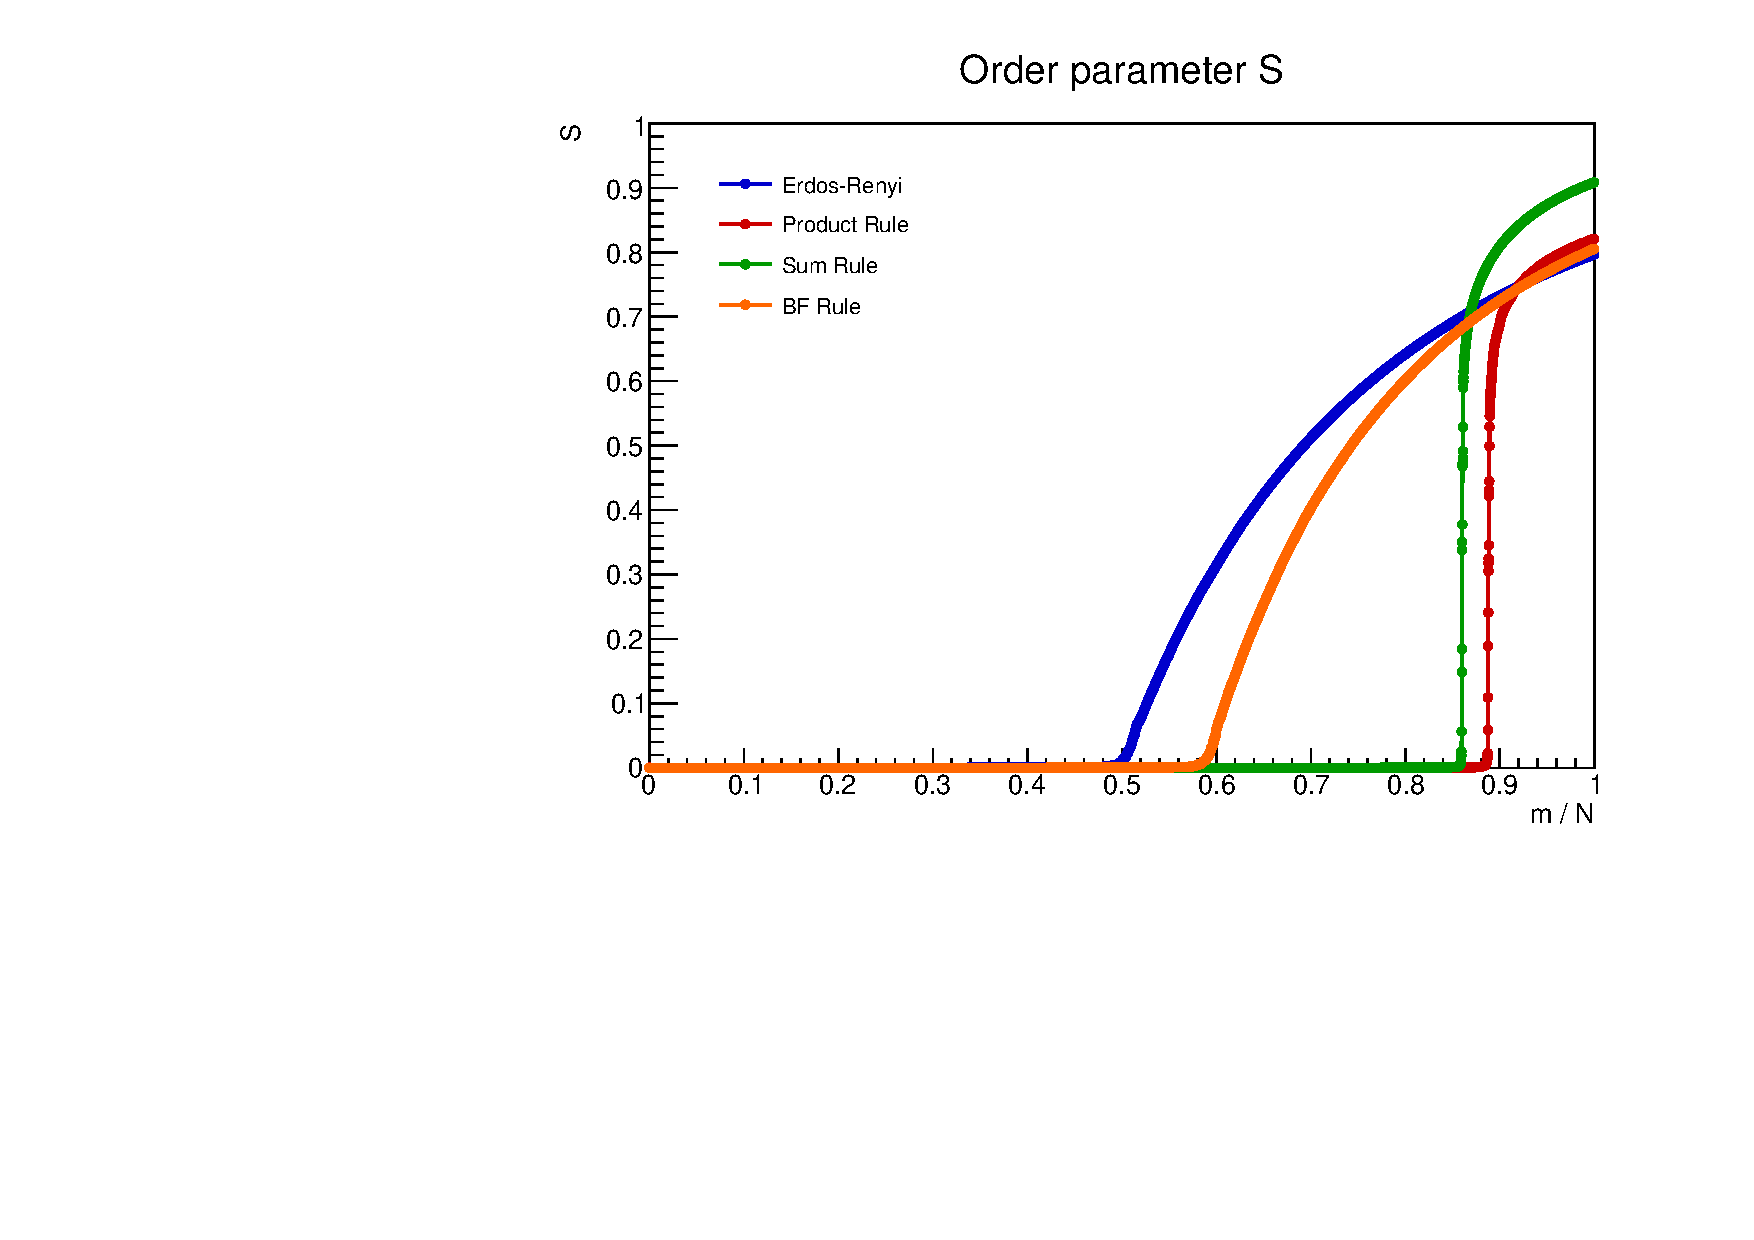
\includegraphics[width=\linewidth]{images/S.pdf}
		\vspace{-28pt}
		\caption{}
		\label{fig::S}
	\end{subfigure}
	\hspace{3pt}
	\begin{subfigure}[t]{0.48\linewidth}
		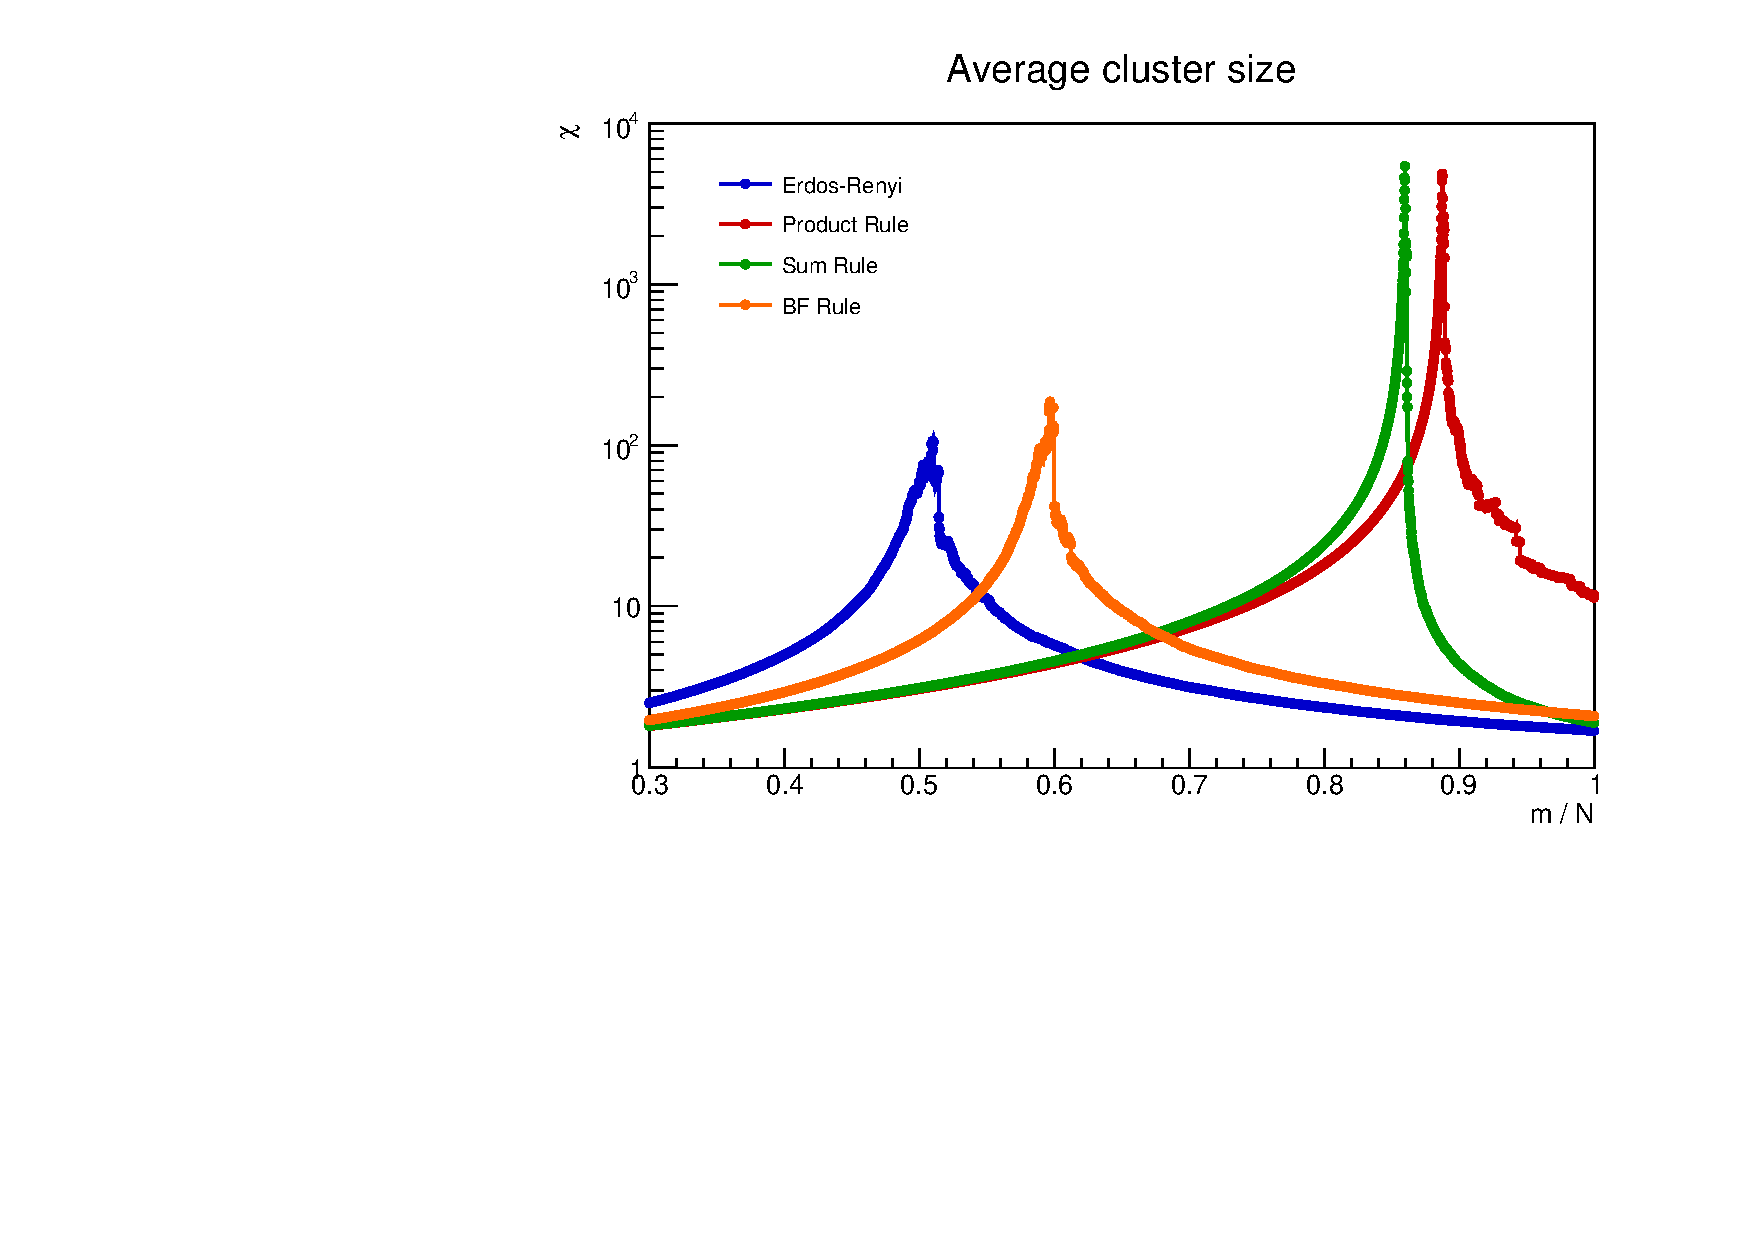
\includegraphics[width=\linewidth]{images/ACS.pdf}
		\vspace{-28pt}
		\caption{}
		\label{fig::ACS}
	\end{subfigure}
	\vspace{-10pt}
	\caption{\textit{(a) LCC size vs.\ added edges $m/N$, $N = 10^6$. Both ER and BF protocol give rise to a continuous phase transition, while competitive rule like PR and SR generates a seemingly looking discontinuous PT (b) Average cluster size vs.\ $m/N$, $N = 10^6$.}}
	\vspace{-8pt}
\end{figure}


\section{Explosive percolation in SF networks}
\label{par::SF}
We now turn our attention to a different network topology, i.e. scale-free networks whose degree distribution $P(k) \sim k^{-\gamma}$, using a configuration model. We proceed as illustrated in \cite{Radicchi}. Let $N$ be the initial number of initially disconnected nodes. Sampling from a power law, we associate to each node a fixed amount of stubs and we gradually proceed to connect them following either a PR rule or a random choice (of course, when connecting stubs at random we fall back on the classical percolation problem on scale-free networks). Results for $S$ are shown in Fig \ref{fig::RGSF}, \ref{fig::PRSF}. When performing a random connection between stubs (classical percolation on SF networks), one should expect to see a critical behaviour only when $\gamma > 3$, since $\kappa \to \infty$ for $\gamma < 3$, regardless of $k_{min}$. In fact, when $\gamma < 3$, the order parameter smoothly increases and is $0$ only when $m = 0$. When using PR rule, we observe again the abrupt change when $m \approx m_c(\gamma)$ 

The most interesting result is, however, that using PR for $\gamma = 2.6 < 3$ a phase transition is observed. In fact, one can show \cite{Radicchi}, \cite{Cho_2009} that, when using PR, the threshold below which the GCC is always observed (thus no PT) is $\gamma = \gamma_c \approx 2.4$. When $\gamma > \gamma_c$, a steep PT is measured. However, as already mentioned, looks can be deceiving: even if highly abrupt, those PTs are still of the second order. 

\begin{figure}[H]
	\centering
	\begin{subfigure}[t]{0.48\linewidth}
		\includegraphics[width=\linewidth]{images/S_SF.pdf}
		\vspace{-28pt}
		\caption{}
		\label{fig::RGSF}
	\end{subfigure}
	\hspace{3pt}
	\begin{subfigure}[t]{0.48\linewidth}
		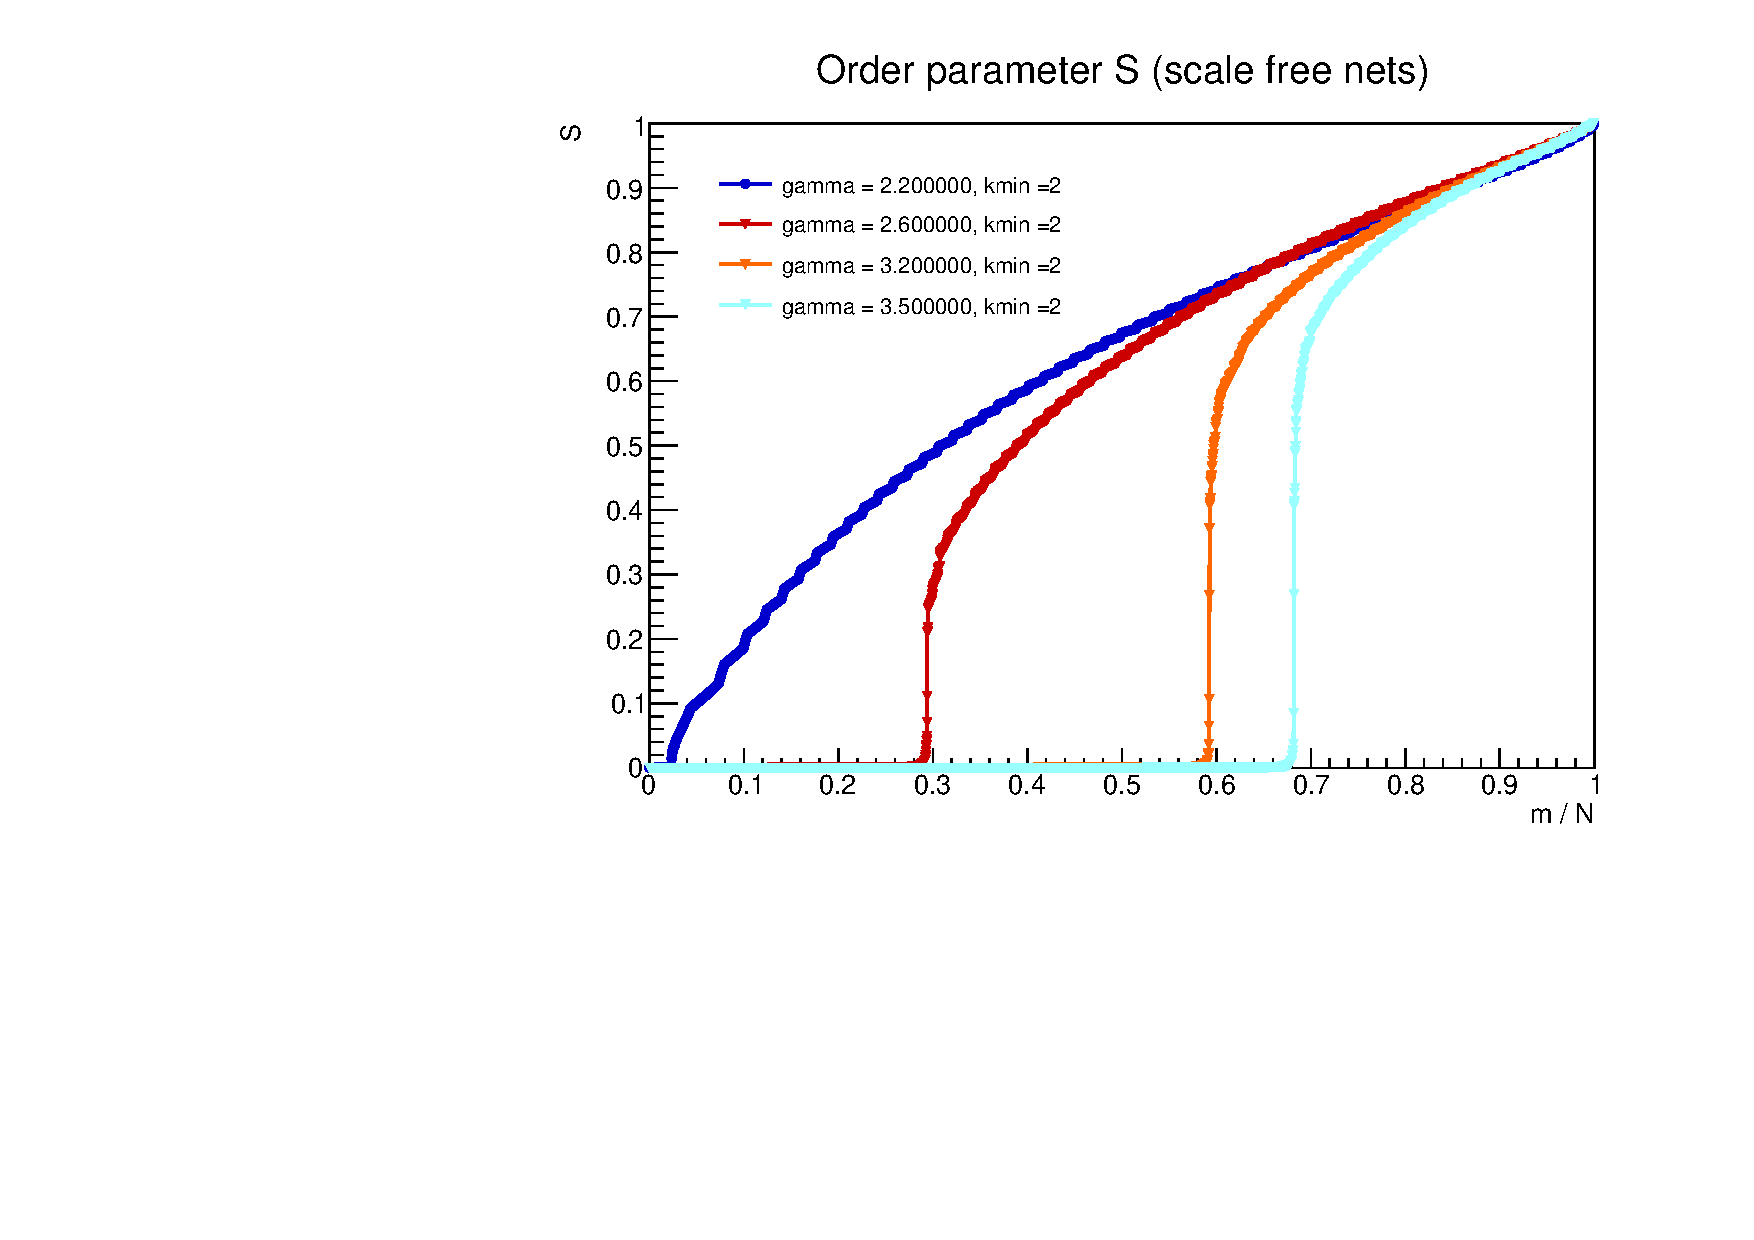
\includegraphics[width=\linewidth]{images/S_PR.pdf}
		\vspace{-28pt}
		\caption{} 
		\label{fig::PRSF}
	\end{subfigure}
	\vspace{-10pt}
	\caption{\textit{(a) LCC size vs. added edges $m/N$, $N = 10^6$, randomly connecting stubs until a power law is reached (classical percolation on SF networks)} (b) \textit{LCC size vs.\ added edges $m/N$, $N = 10^6$, using PR rule to connect stubs. Averages on $10$ independent realizations}}
\end{figure}
\newpage

\section{Supplementary material}
\subsection{Scaling law for $\Delta m$}
\label{par:scaling}
In its seminal work \cite{Achlioptas}, Achlioptas proposes an operational method to decide whether the observed PT is continuous or discontinuous. Consider again the procedure presented in Par. \ref{par:Achlioptas}, where edges are gradually added $m = m(t) = t$ following different protocols (ER, PR, SR, BF) and the LCC size is monitored. We will define two edge value $m_0$ and $m_1$ at different times such that:
\begin{equation}
	\begin{cases}
		m_0 = \min_{m < M}\{S > \sqrt{N}\} \\
		m_1 = \min_{m < M}\{ S > 0.5 N\} 
	\end{cases}
\end{equation}
The difference $\Delta$, called transition window, is defined as $\Delta = m_1 - m_0$ and provide a quantitative way to define how abrupt the PT is\footnote{The choice of the endpoints is, up to a certain extent, arbitrary. The value of $m_0$ is chosen because, usually, at criticality the LCC scale logarithmically with $N$, and thus provides an estimate of the critical point}.  

As claimed in \cite{Achlioptas}, $\Delta$ should scale linearly for continuous PTs, $\Delta \sim N$. So by observing the scaling behaviour of $\Delta$ in simulations, one can characterize a bit further the PT. Results are shown in Fig. \ref{fig::ScalingDelta}. For both ER and BF rule, $\frac{\Delta }{N}$ seems indeed to converge to a finite value when $N$ is large enough and the results we obtained are compatible with Achlioptas' findings. At variance, when using PR or SR rule, the curves tend to collapse at $0$, suggesting a sub-linear behaviour. And in fact, plotting $\frac{\Delta}{N^{\alpha}}$ with $\alpha = \frac{2}{3}$ (Fig. \ref{fig::ScalingDelta23}), results from PR and SR now stabilizes to a small but different from $0$ value (again, in agreement with \cite{Achlioptas}). This means that explosive percolation is characterized by a sub-linear scaling law of the critical window:
$$
\Delta \sim N^{\frac{2}{3}}
$$
If $m_0$ is interpreted as an estimate of the critical point and $m_1$ a point where the GCC has already emerged, than one can say that the distance between the percolating phase and the critical point gets smaller and smaller when $N \to \infty$. 
This implies that, at criticality, a constant fraction of the vertices is accumulated into a single giant cluster within a sub-linear number of steps \cite{BOCCALETTI20161}

However, in 2009, Ziff \cite{Ziff} showed that, for the regular percolation on a 2D lattice, $\Delta \sim N^{\alpha}$ with $\alpha \neq 1$, so this is not conclusive evidence that explosive percolation is a discontinuous PT.
It is today accepted that EP under Achlioptas processes are actually continuous PTs, but with a universality class
different from all the others percolative processes.
\begin{figure}
	\centering
	\begin{subfigure}[t]{0.48\linewidth}
		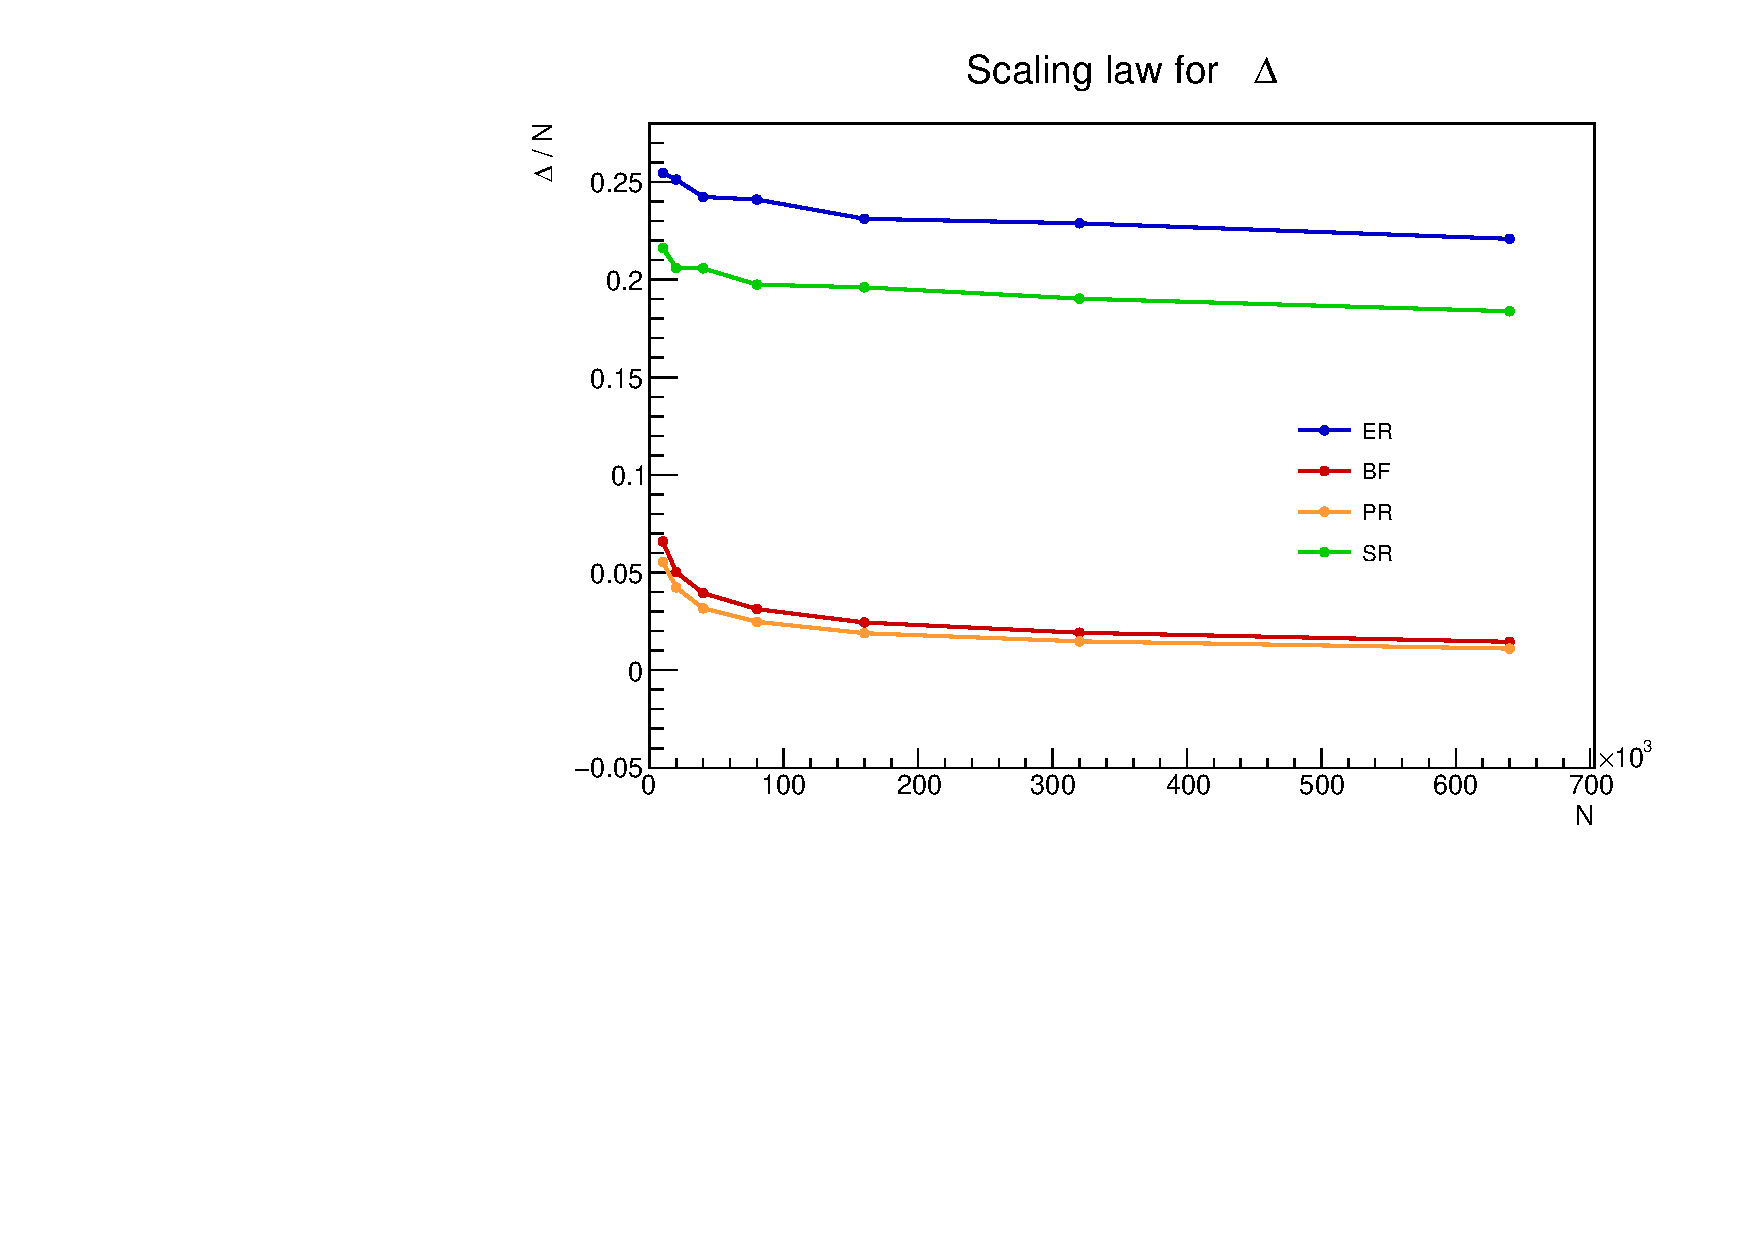
\includegraphics[width=\linewidth]{images/ScalingLaw.pdf}
		\vspace{-28pt}
		
		\caption{}
		\label{fig::ScalingDelta}
	\end{subfigure}
	\hspace{3pt}
	\begin{subfigure}[t]{0.48\linewidth}
		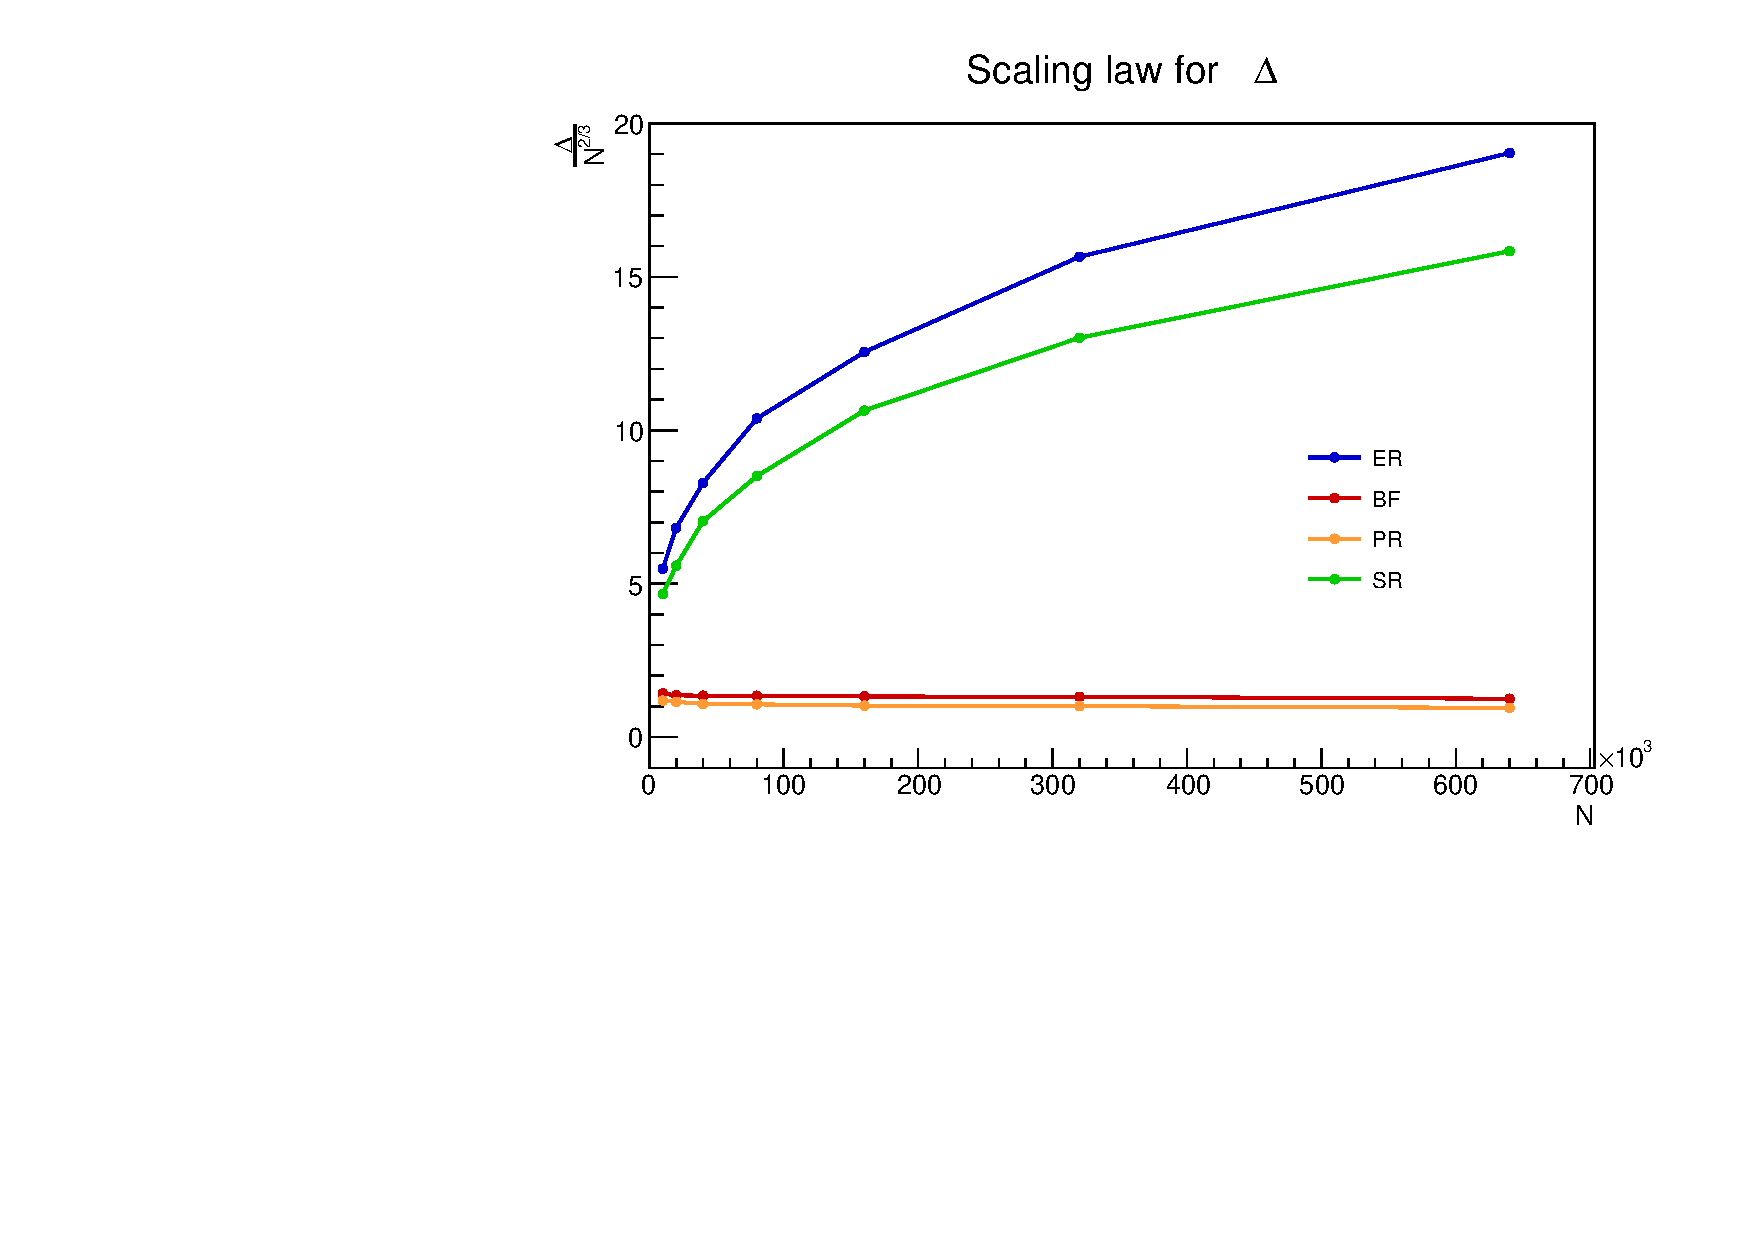
\includegraphics[width=\linewidth]{images/ScalingLaw23.pdf}
		\vspace{-28pt}
		\caption{} 
		\label{fig::ScalingDelta23}
	\end{subfigure}
	\vspace{-10pt}
	\caption{\textit{(a) LCC size vs. added edges $m/N$, $N = 10^6$, randomly connecting stubs until a power law is reached (classical percolation on SF networks)} (b) \textit{LCC size vs.\ added edges $m/N$, $N = 10^6$, using PR rule to connect stubs. Averages on $10$ independent realizations}}
\end{figure}

\subsection{Cluster size distribution}
Let us investigate further the behaviour of the cluster size distribution of continuous PTs. Defining $n_s$ as the number of clusters of size $s$ per node, then out of criticality $n_s$ has exponentially distributed tails. When approaching the critical point, the distribution becomes a power law
$$
n_s \sim s^{-\tau}  \mbox{ for large }s 
$$
where $\tau$ is usually called the Fisher exponent. This power law is another strong indicator of the onset of a second order PT.

Thus, we can collect the cluster distribution $n_s$ at different value of $m / N$ (centered around the critical point). Results carried out for each percolative process as those presented in Par. \ref{par:Achlioptas} (Erdos-Renyi, Product Rule, Sum Rule, BF rule) are shown in Fig. \ref{fig:ClusterDistr}. And indeed, when $m \sim m_c$, the distribution gets closer and closer to a power law (a straight line in a log-log plot) in all cases, providing more evidence that explosive percolation is a continuous PT.
\label{par:css}
\begin{figure}
	\centering
	\begin{subfigure}[b]{0.48\linewidth}
		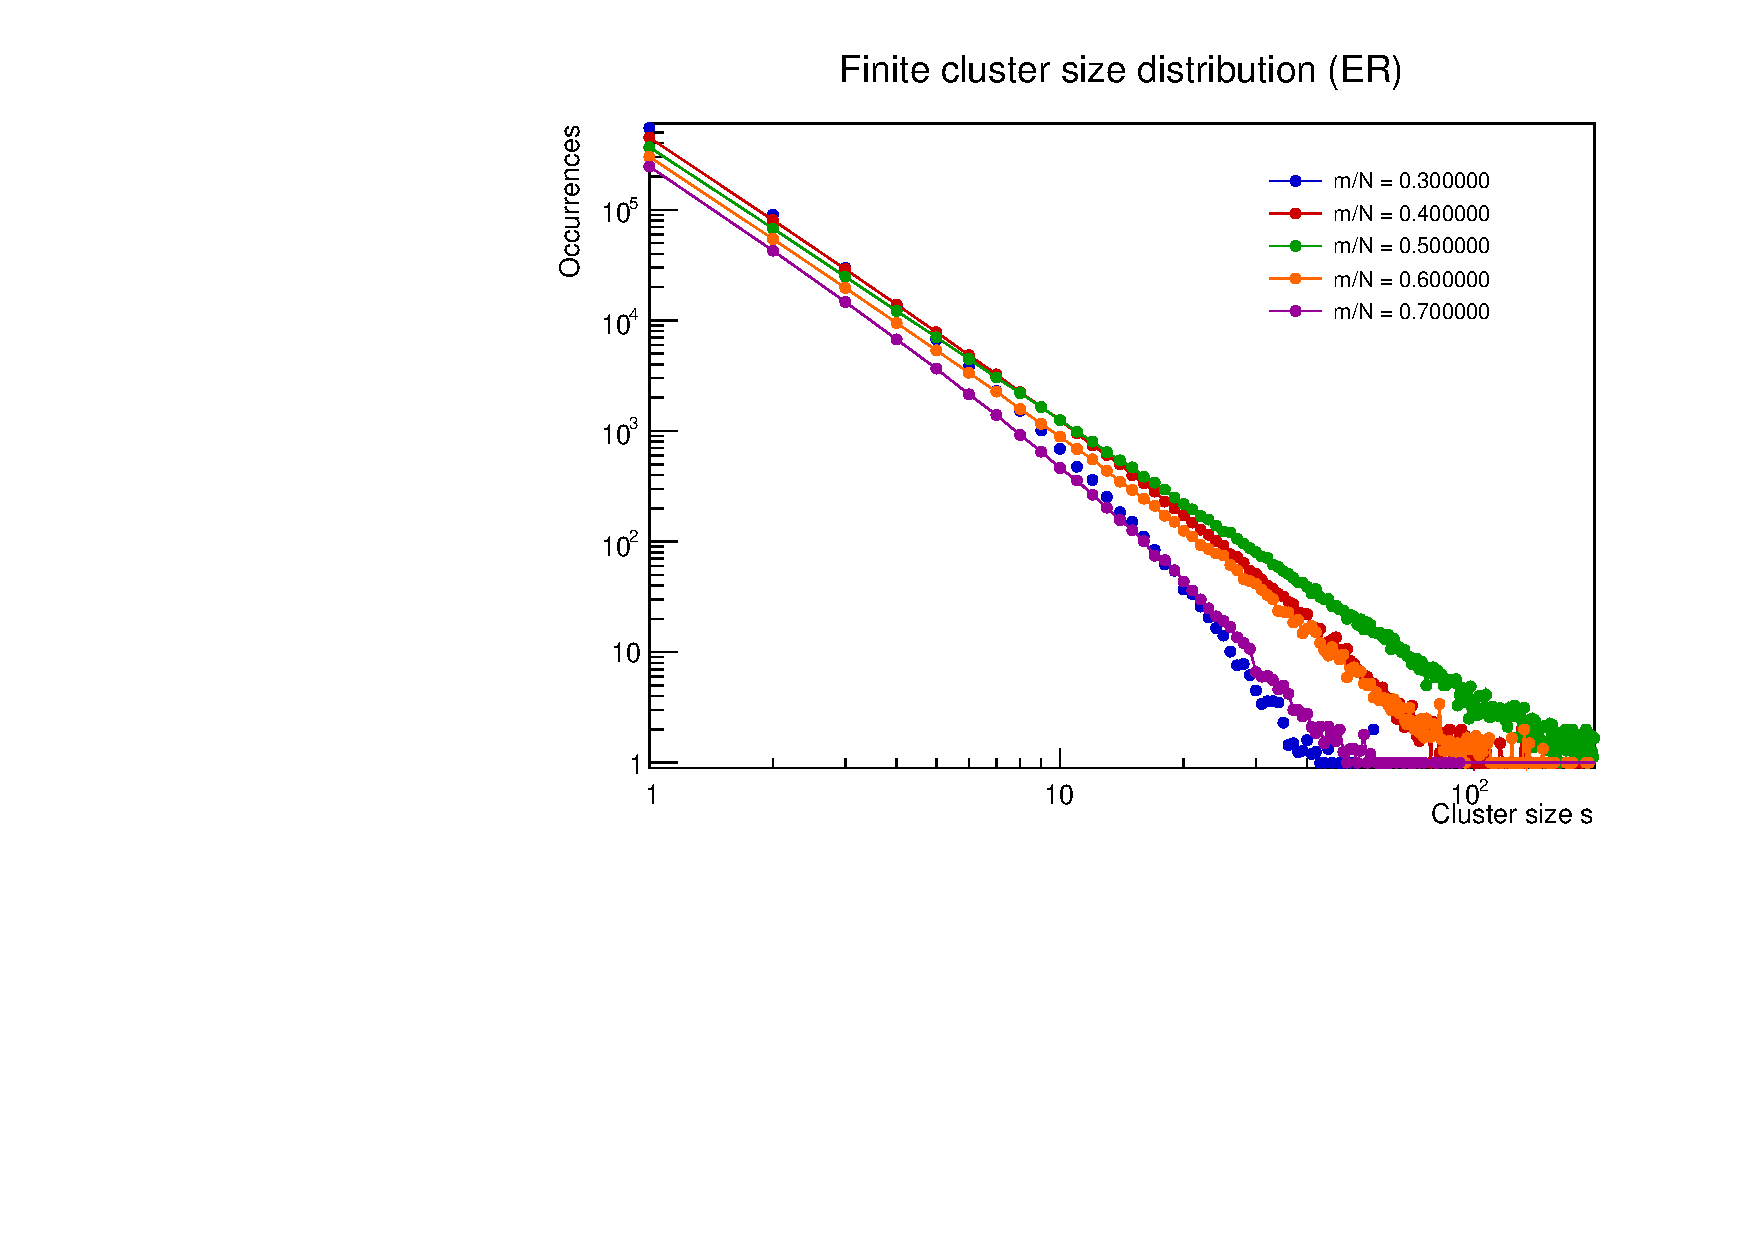
\includegraphics[width=\linewidth]{images/ClusterDistrER.pdf}
	\end{subfigure}
	\hspace{0.5em}
	\begin{subfigure}[b]{0.48\linewidth}
		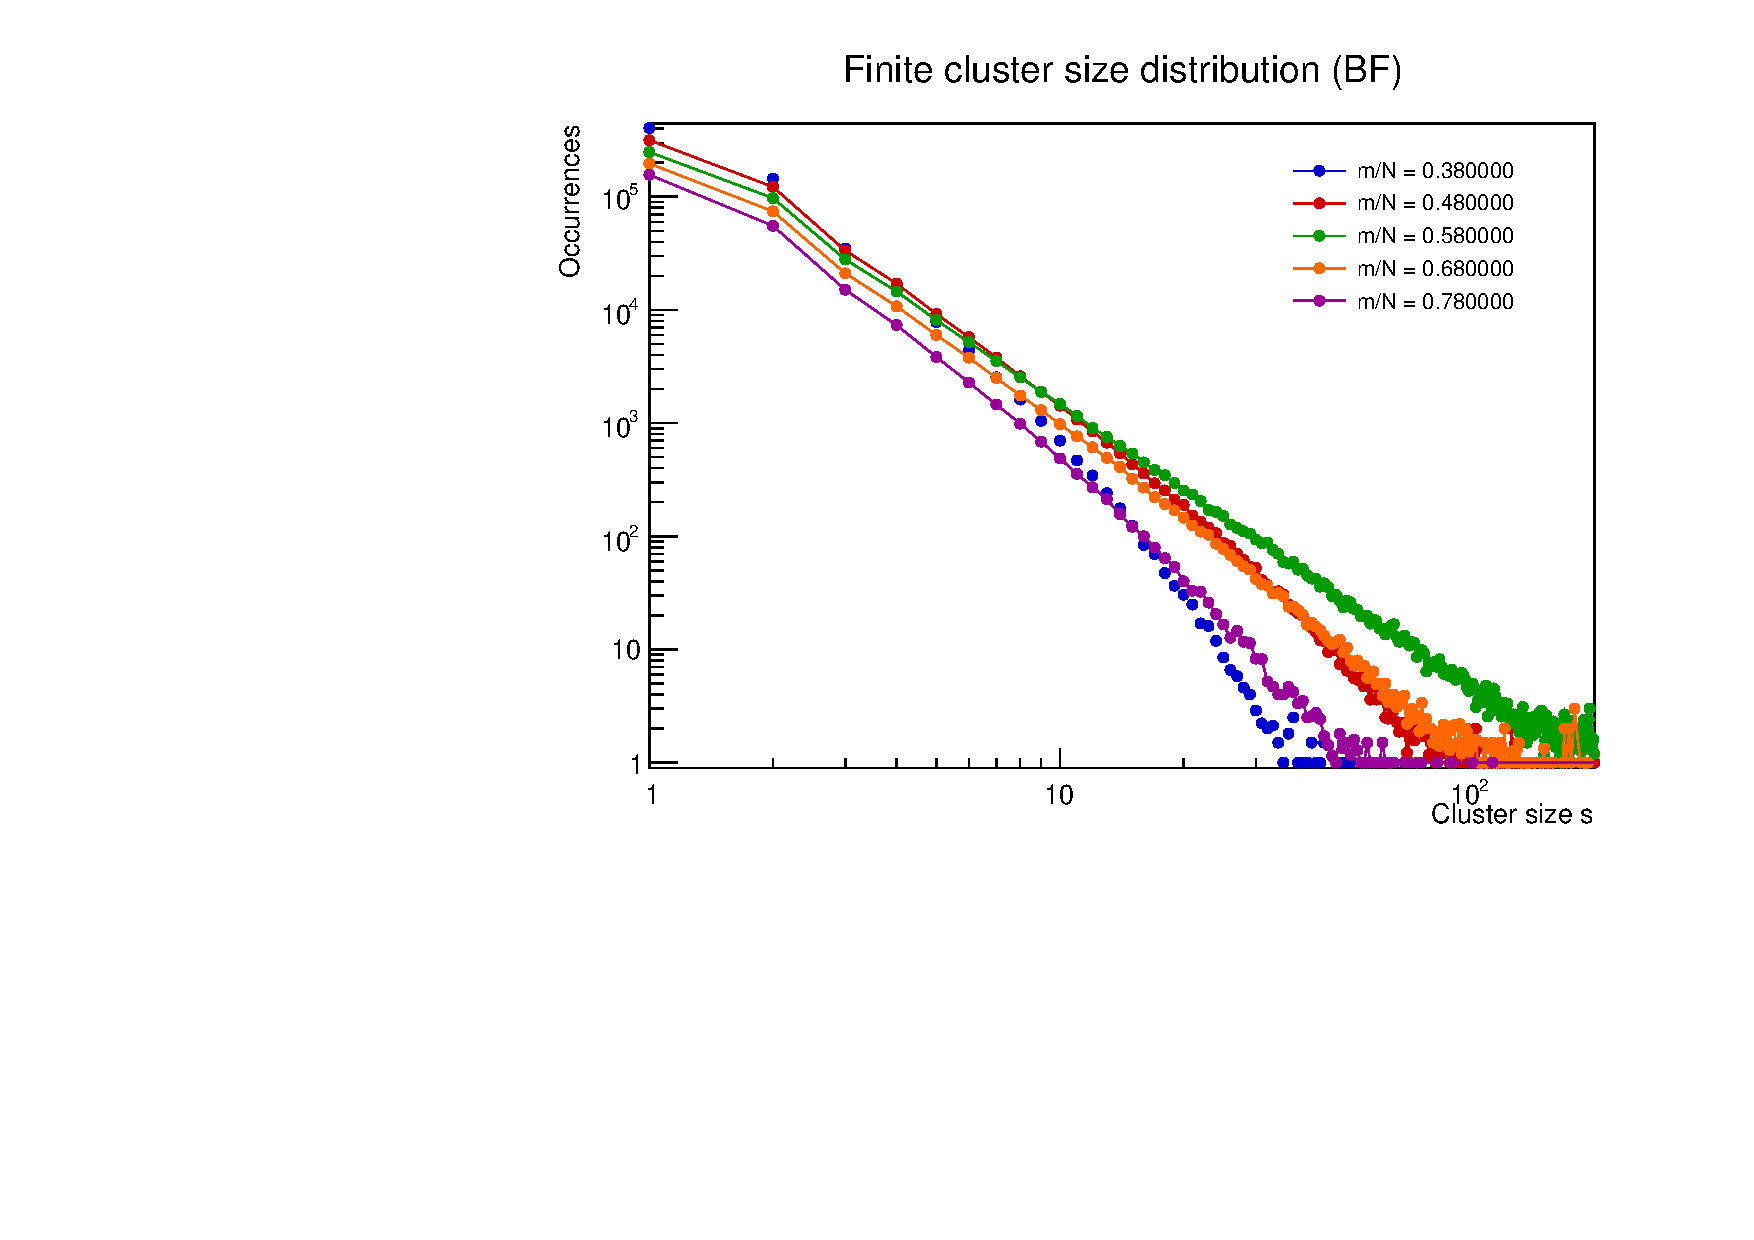
\includegraphics[width=\linewidth]{images/ClusterDistrBF.pdf}
	\end{subfigure}
	
	\vspace{0.5em} % Spazio tra righe
	
	\begin{subfigure}[b]{0.48\linewidth}
		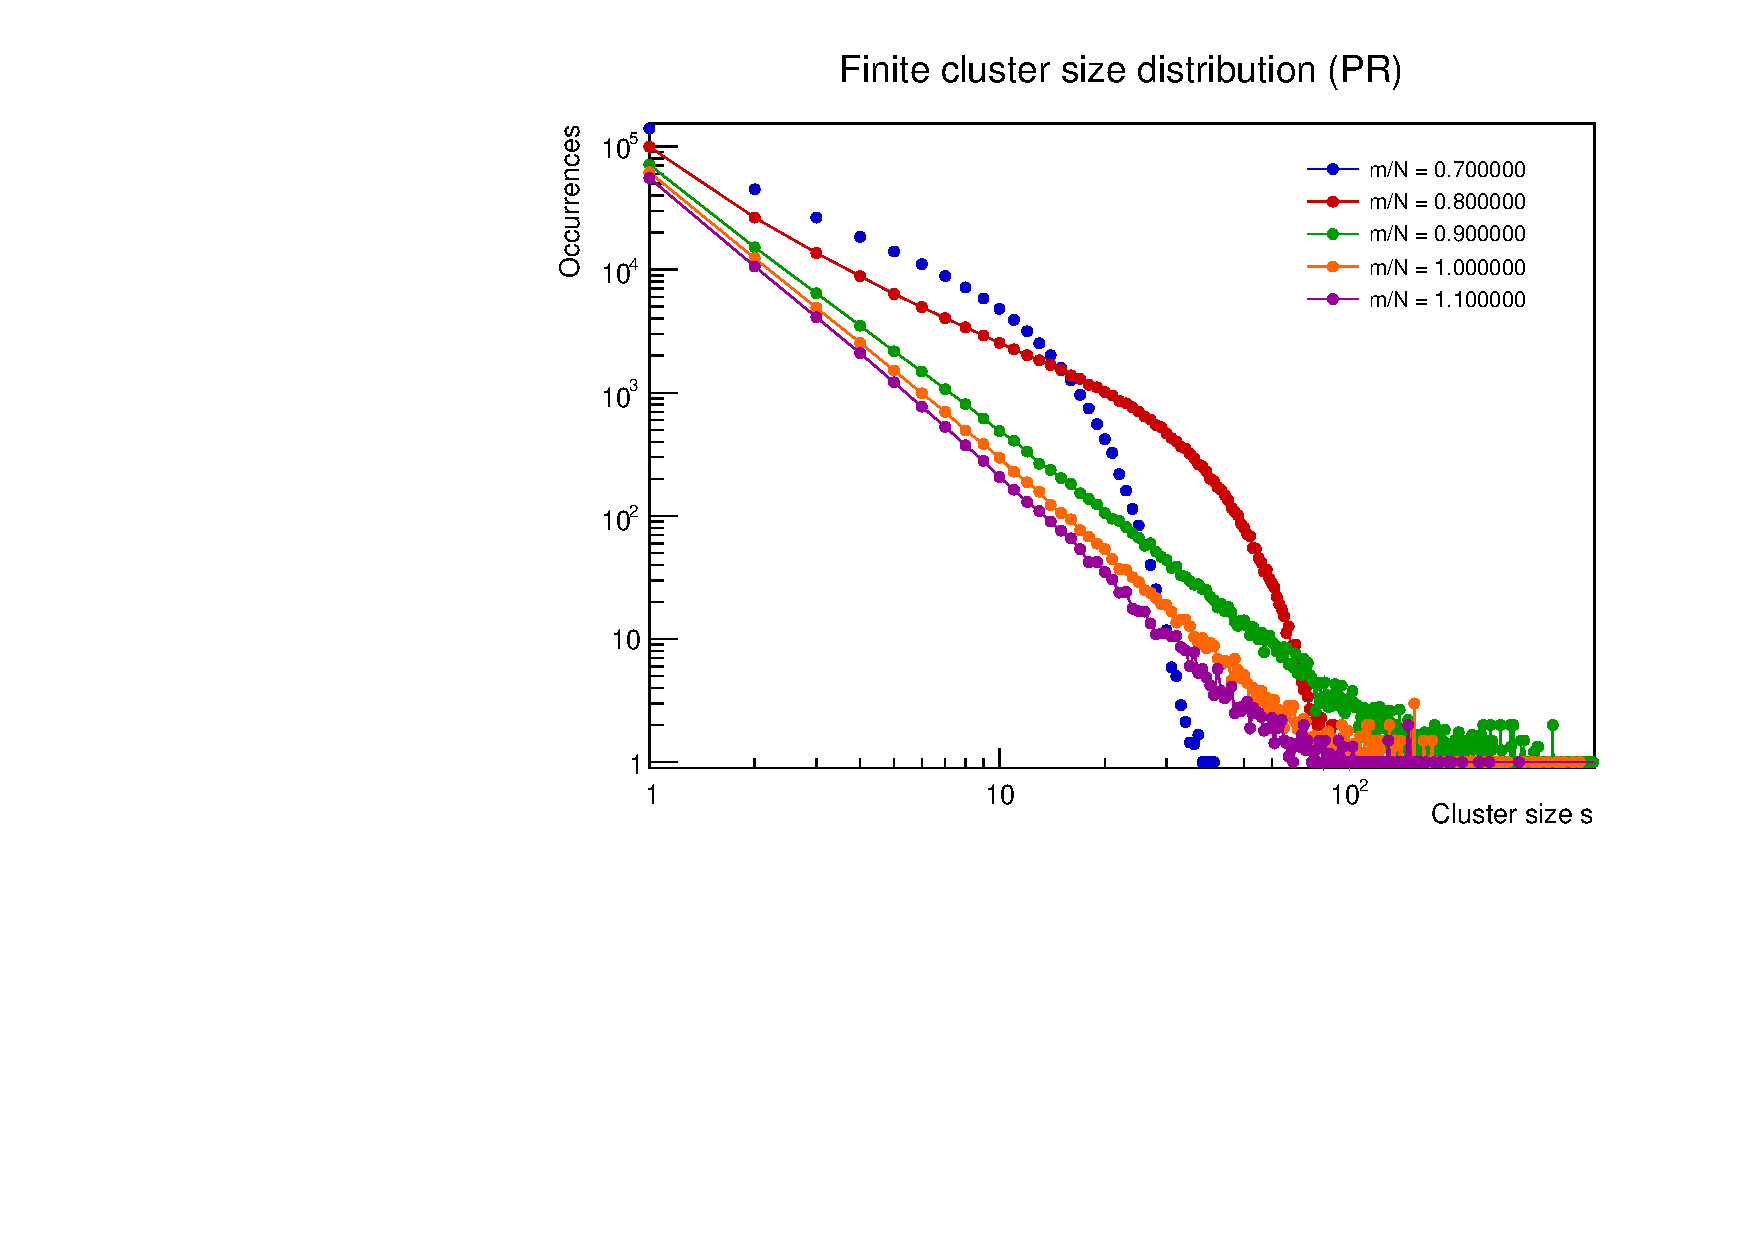
\includegraphics[width=\linewidth]{images/ClusterDistrPR.pdf}
	\end{subfigure}
	\hspace{0.5em}
	\begin{subfigure}[b]{0.48\linewidth}
		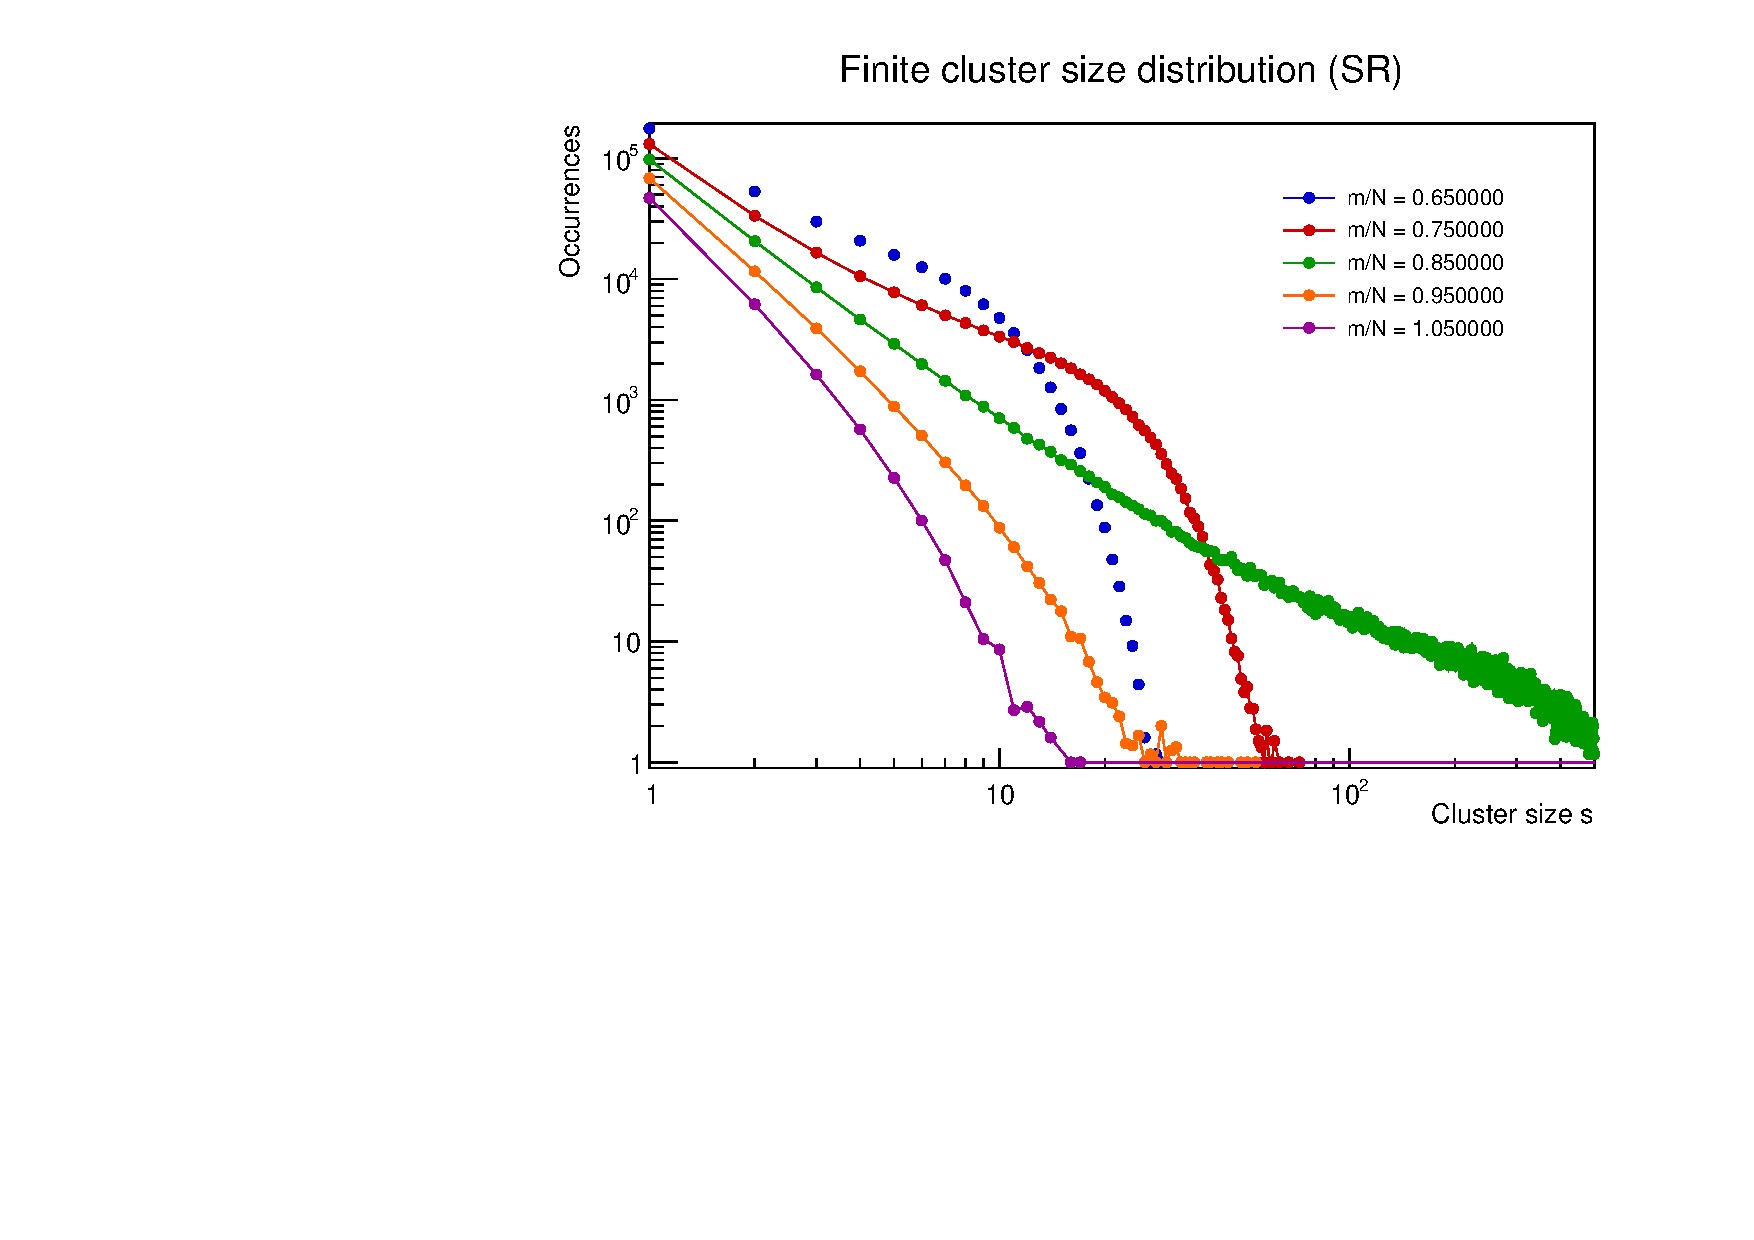
\includegraphics[width=\linewidth]{images/ClusterDistrSR.pdf}
	\end{subfigure}
	\caption{\textit{Finite cluster size distribution at and around criticality. As expected, when $m \approx m_c$, the distribution appears approximately as a power law (the critical value can be estimated inspecting Fig.\ref{fig::S}). Simulation run on networks with $N = 10^6$, over $10$ independent realizations}}
	\label{fig:ClusterDistr}
\end{figure}

\subsection{Again on SF networks}
In Par.\ref{par::SF}, explosive percolation was presented on scale-free networks. In this appendix, we are going to show more processed data and explain the theoretical framework behind SF networks.

Using our configuration model, we will impose a discrete degree distribution $P(k)$:
\begin{equation}
	P(k) = \frac{1}{Z} k^{-\gamma}
	\label{eq:Het}
\end{equation}
To normalize it, we need to set at least two boundaries, $k_{min}, k_{max}$. We choose $k_{max} = k_{min} N^{\frac{1}{\gamma - 1}}$, i.e. the natural cutoff and $k_{min}$ is a free parameter. As $N \to \infty$, we can assume $k_{max} = \infty$ for computations purposes. 

For uncorrelated networks, the presence of a GCC is conditioned to the Molloy-Reed coefficient $\kappa$:
$$
\kappa = \frac{\langle k^2 \rangle}{\langle k \rangle}
$$
Using Eq. \ref{eq:Het}, we can compute the statistical moments. Setting $k_{min}=1$:
\begin{equation}
	\begin{aligned}
		\langle k^2 \rangle = \frac{1}{Z} \sum_{k_{min}}^{\infty} k^{2-\gamma} = \frac{\zeta(\gamma-2)}{\zeta(\gamma)}  \\
		\langle k \rangle = \frac{1}{Z} \sum_{k_{min}}^{\infty} k^{1-\gamma} = \frac{\zeta(\gamma-1)}{\zeta(\gamma)}  \\
	\end{aligned}
\end{equation}
whereas, for $k_{min} = 2$, 

\begin{equation}
\begin{aligned}
	\langle k^2 \rangle = \frac{1}{Z} \sum_{k_{min}}^{\infty} k^{2-\gamma} = \frac{\zeta(\gamma-2)-1}{\zeta(\gamma)-1}  \\
	\langle k \rangle = \frac{1}{Z} \sum_{k_{min}}^{\infty} k^{1-\gamma} = \frac{\zeta(\gamma-1)-1}{\zeta(\gamma)-1}  \\
\end{aligned}
\end{equation}
So that, finally,
\begin{equation}
	\kappa_1 = \frac{\zeta(\gamma-2)}{\zeta(\gamma)} \>\>\>\>\>\>  \kappa_2 = \frac{\zeta(\gamma-2)-1}{\zeta(\gamma)-1}
\end{equation}
The critical point for uncorrelated networks can be computed as:
\begin{equation}
	\label{eq:Critical}
	p_c = \frac{1}{\kappa - 1}
\end{equation}
If $\gamma < 3$, then $\zeta(\gamma-2)$ diverges to infinity and $p_c = 0$, so technically there is no critical behaviour and a GCC always exists, even with low connectivity. When $\gamma > 3$, a GCC finally appears together with a PT at a fixed $p_c$. However, for the GCC to be there even when $p_c = 1$ (full network recovered), then $\kappa > 2$. One can easily show that, when selecting $k_{min} = 1$:
\begin{itemize}
		\item $\gamma < 3$: $\kappa = \infty$ and $p_c = 0$. The GCC is always present and is $0$ only when $p_c = 0$.
		\item $3 < \gamma < \gamma_c \approx 3.5$: $2 < \kappa < \infty $. The system displays two phases (percolating and non percolating) separated by a critical point
		\item $\gamma > \gamma_c$: $\kappa < 2$. Even at full connectivity, there's no GCC so it makes no sense to talk about a PT here
\end{itemize}

Running a classical percolation on a SF networks, we got the results presented in Fig. \ref{fig::RGSF1}. They are compatible with our theoretical understanding of the process. The dotted line represents the analytically computed value of $p_c = m_c / M$ ($M$ being the total number of generated stubs divided by $2$). Its value is not too accurate and this is probably due to the fact that $k_{max}$ was not set to infinity but to a large finite value. Indeed, we can compute directly from the generated distribution of the stubs the value of $\kappa$ and use this value in Eq. \ref{eq:Critical} rather then computing it analytically. If we do so, we obtain better and more realistic result

When $k_{min} = 2$, then $\kappa > 2, \>\> \forall \gamma > 3$. Plots regarding the behaviour of $S$ for regular percolation when $k_{min}$ are shown in Fig. \ref{fig::RGSF2}. Now, we see the formation of a GCC and a PT even when $\gamma = 3.8$ (which was not the case when $k_{min} = 1$). This justifies our choice of selecting $k_{min} = 2$ in Par. \ref{par::SF}

\begin{figure}
	\centering
	\begin{subfigure}[t]{0.8\linewidth}
		\includegraphics[width=\linewidth]{images/RGSF_kmin1.pdf}
		\vspace{-28pt}
		
		\caption{}
		\label{fig::RGSF1}
	\end{subfigure}
	\hspace{3pt}
	\begin{subfigure}[t]{0.8\linewidth}
		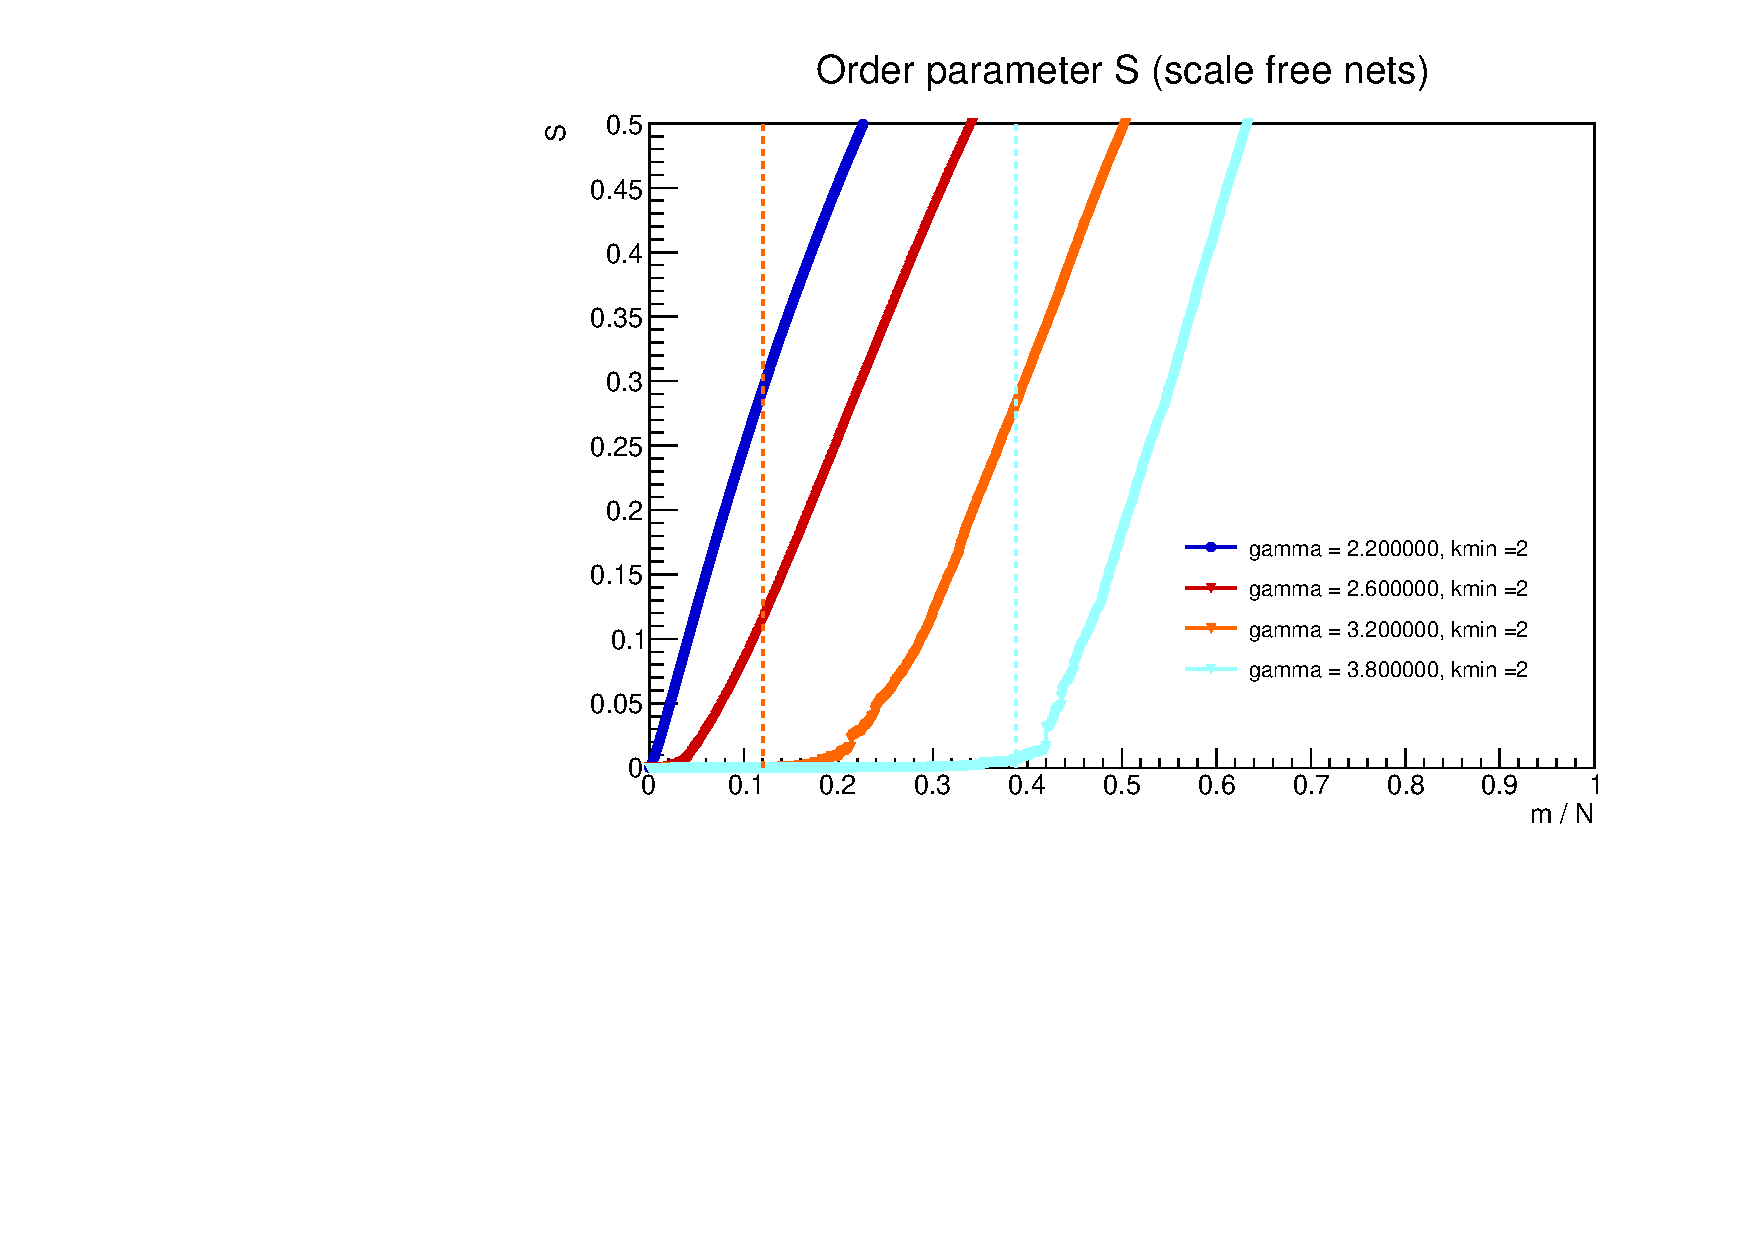
\includegraphics[width=\linewidth]{images/RGSF_kmin2.pdf}
		\vspace{-28pt}
		\caption{} 
		\label{fig::RGSF2}
	\end{subfigure}
	\vspace{-10pt}
	\caption{\textit{(a) Classical random percolation on SF networks when $k_{min} = 1$ and for various value of $\gamma$. Only when $\gamma = 3.2$ do we see a PT. The dotted line represent the critical point as computed in Eq. \ref{eq:Critical}. (b) Classical random percolation on SF networks, $k_{min}$ = 2. Now $\gamma = 3.8$ too displays a PT and a GCC. Dotted lines represent the critical point as computed in Eq. \ref{eq:Critical}}}
\end{figure}


\newpage